\section{Code Base}
\label{appendix:code-base}
All code utilized in this project can be found at https://github.com/rohanbansal12/extended\_essay. Both approaches, \acrlong{rfs} and \acrshort{bert}, have their own folders in the repository. Crawling/Scraping scripts can be found in the data-collection folder. The files used to build this paper in \LaTeX\ are found in the EE folder. I have included certain examples and relevant scripts throughout the paper and appendices. 

\section{Crawling Scripts}
\label{appendix:crawling}
A few sample crawling scripts that were utilized have been included.
\subsection{Longform.org Crawling Script}
\begin{minted}{python}
@dataclass_json
@dataclass
class LongformArticleUrl:
    url: str
    title: str
    source: str

class WriteThread(Thread):
    def __init__(self, queue: Queue, *args, **kwargs):
        super().__init__(*args, **kwargs)
        self.queue = queue
	def run(self):
        with open(OUTPUT_FILE, 'a') as output_file:
            output_file.write("[\n")
            first_entry = True
			while True:
			    article = self.queue.get()
				if article is None:
			        output_file.write("\n]")
			        break
				article_json = article.to_json(indent=4)
				if first_entry:
			        first_entry = False
			    else:
			        output_file.write(",\n")
				output_file.write(article_json)

class ScrapeThread(Thread):
    def __init__(self, chunk, queue: Queue, *args, **kwargs):
        super().__init__(*args, **kwargs)
        self.chunk = chunk
        self.queue = queue
	def run(self):
        for i in self.chunk:
            try:
                print(f'Getting articles from list page {i}')
                article_list_page = get(f"{BASE_URL}{i}")
                soup = BeautifulSoup(article_list_page.text, "html5lib")
                articles = soup.find_all('article', 
                    {'class': 'post--single'})
                for article in articles: 
                    link = article.find('a', 
                        {'class': 'post__link'})
                    title = article.find('span', 
                        {'class': 'post__title__highlight'})
                    source = article.find('a', 
                        {'class': 'post__permalink'})
                    print(link)
                    if (title is None or 
                        title.string is None or 
                        source is None):
                        continue
                    article_url = LongformArticleUrl(url=link['href'], 
                        title=str(title.string.strip()) or '', 
                        source=source['href'])
                    self.queue.put(article_url)
            except Exception as e:
                print(f'Something went wrong when scraping: {e}')
                print("------------------------------------------")
\end{minted}
\subsection{Vox Crawling Script}
\begin{minted}{python}
@dataclass_json
@dataclass
class VoxArticleUrl:
    url: str
    title: str
    month: int
    year: int

YEARS = [str(month) for month in range(2014,2020)]
MONTHS = [str(month) for month in range(1,13)]

class WriteThread(Thread):
    def __init__(self, queue: Queue, *args, **kwargs):
        super().__init__(*args, **kwargs)
        self.queue = queue

    def run(self):
        with open(OUTPUT_FILE, 'a') as output_file:
            output_file.write("[\n")
            first_entry = True
            while True:
                article = self.queue.get()
                if article is None:
                    output_file.write("\n]")
                    break
                article_json = article.to_json(indent=4)
                if first_entry:
                    first_entry = False
                else:
                    output_file.write(",\n")
                output_file.write(article_json)


class ScrapeThread(Thread):
    def __init__(self, chunk, queue: Queue, *args, **kwargs):
        super().__init__(*args, **kwargs)
        self.chunk = chunk
        self.queue = queue
    def get_urls(self, year, month):
        page = 1
        while True:
            sleep(1)  # Prevent rate limiting
            print(f'Getting articles for {year}-{month}, page {page}')
            return_data = get(f"{BASE_URL}/{year}/{month}/{page}", 
                headers={'Accept': 'application/json'})
            if return_data.status_code != 200:
                print(f"Received status {return_data.status_code}")
                if return_data.status_code != 429:
                    return
                else:
                    sleep(10)
            else:
                page = page + 1
                response = return_data.json()
                soup = BeautifulSoup(response['html'], 
                    "html5lib")
                yield soup
                if not response['has_more']:
                    break
    def run(self):
        for year, month in self.chunk:
            try:
                for html in self.get_urls(year, month):
                    h2s = html.find_all('h2')
                    for h2 in h2s:
                        a = h2.find('a')
                        title = a.string
                        url = a['href']
                        print(title,url)
                        vox_url = VoxArticleUrl(title=str(title), 
                            url=str(url), 
                            month=int(month), 
                            year=int(year))
                        self.queue.put(vox_url)
            except Exception as e: # Best effort
                print(f'Something went wrong when scraping: {e}')
\end{minted}

\section{Scraping Scripts}
\label{appendix:scraping}
The majority of the scraping utilized the same code for all sources, in contrast to the crawling scripts, which were based on the specific HTML layout of the websites. I did utilize an alternative method for difficult to scrape sites, and both are presented here.
\subsection{Vanilla Scraping Script}
\begin{minted}{python}
import json
from dataclasses import dataclass, field
from dataclasses_json import dataclass_json
from datetime import datetime
from newspaper import Article
from bs4 import BeautifulSoup
from typing import List
from queue import Queue
from threading import Thread

@dataclass_json
@dataclass
class LongformArticle:
    title: str = ''
    text: str = ''
    url: str = ''
    source: str = ''

class WriteThread(Thread):
    def __init__(self, queue: Queue, *args, **kwargs):
        super().__init__(*args, **kwargs)
        self.queue = queue

    def run(self):
        with open(OUTPUT_FILE, 'a') as output_file:
            output_file.write("[\n")
            first_entry = True
            while True:
                article = self.queue.get()
                if article is None:
                    output_file.write("\n]")
                    break
                article_json = article.to_json(indent=4)
                if first_entry:
                    first_entry = False
                else:
                    output_file.write(",\n")
                    output_file.write(article_json)


class ScrapeThread(Thread):
    def __init__(self, urls, queue: Queue, *args, **kwargs):
        super().__init__(*args, **kwargs)
        self.urls = urls
        self.queue = queue
    @staticmethod
    def scrape(url):
        article = Article(url['url'])
        article.download()
        article.parse()
        soup = BeautifulSoup(article.html, 'lxml')
        ga = LongformArticle()
        ga.url = url['url']
        ga.title = url['title']
        ga.text = article.text
        ga.source = url['source']
        return ga
    def run(self):
        for url in self.urls: 
            try:
                print(f"scraping {url['url']}")
                article = ScrapeThread.scrape(url)
                self.queue.put(article)
            except Exception as e: # Best effort
                print(f'ScrapeThread Exception: {e}')
\end{minted}

\section{Data Processing}
\label{appendix:processing}
I created an Articles class that made dataset handling easy. It includes a built-in mapping function (map\_items), in addition to other methods, such as sampler creations, that were utilized in the rest of the experiment.
The majority of the work necessary for training machine learning models pertains to the actual data being trained on. Many steps are involved in acquiring proper data and cleaning it in a manner that makes training both conducive and effective.

\subsection{Collection}
I began by collecting data from longform.org and longreads.com, which are both publications that scour the web for quality content. The crawling/scraping scripts I wrote and used can be seen in~\Cref{appendix:crawling} and~\Cref{appendix:scraping}. I then asked the CEO of The Browser for his content and he graciously provided access to the company’s archives (refer to~\Cref{appendix:permission}). These articles were combined to be positive examples. To collect negative data, I began with scraping a few major news sites (Vox, Guardian). I then decided to scrape specific publications that frequently appear in the quality writing locations, as these would provide a better test of the models' ability to draw a distinction from content that is actually hand-picked for its writing style. This included sources such as Rolling Stone and Smithsonian Magazine who both focus on longform content. I also decided to use the Fake News Corpus which provides nearly 9 million articles from various fringe parts of the Internet, including hate speech, genuine fake news, and conspiracy theories. These were generally used for non-training purposes to ensure that the model was not susceptible to "bad" content.

\subsection{Cleaning}
The majority of the cleaning and processing was done via the direct crawling/scraping scripts. JSON files were generated for each publication, which included fields for publication, text, and links. The only major caveat with this type of scraping is the possibility for certain sites to detect the script and send back an error message. For this step, I manually checked a few articles from each publication scrape to make sure that proper content was being received by the request. I also filtered out articles that were under 75 words in length as these were primarily error messages or not technically full-length articles.

\subsection{Preparation}
After collection, the text and publication fields had to be mapped to ids for the model. For publications, I mapped all of the quality content I had collected to publication id 0. The remaining publication ids were essentially irrelevant as the model was only relying on the embedding vector for publication 0 to generate predictions. The text needed to be mapped to the corresponding tokens. The tokenizer library from huggingface made this process easy, as it allows for a simple input of a normal sequence of text (in the way that the article content was saved) and generates a dataset of both tokenized words and the corresponding ids which can be observed here:

\begin{figure}[H]
\centering
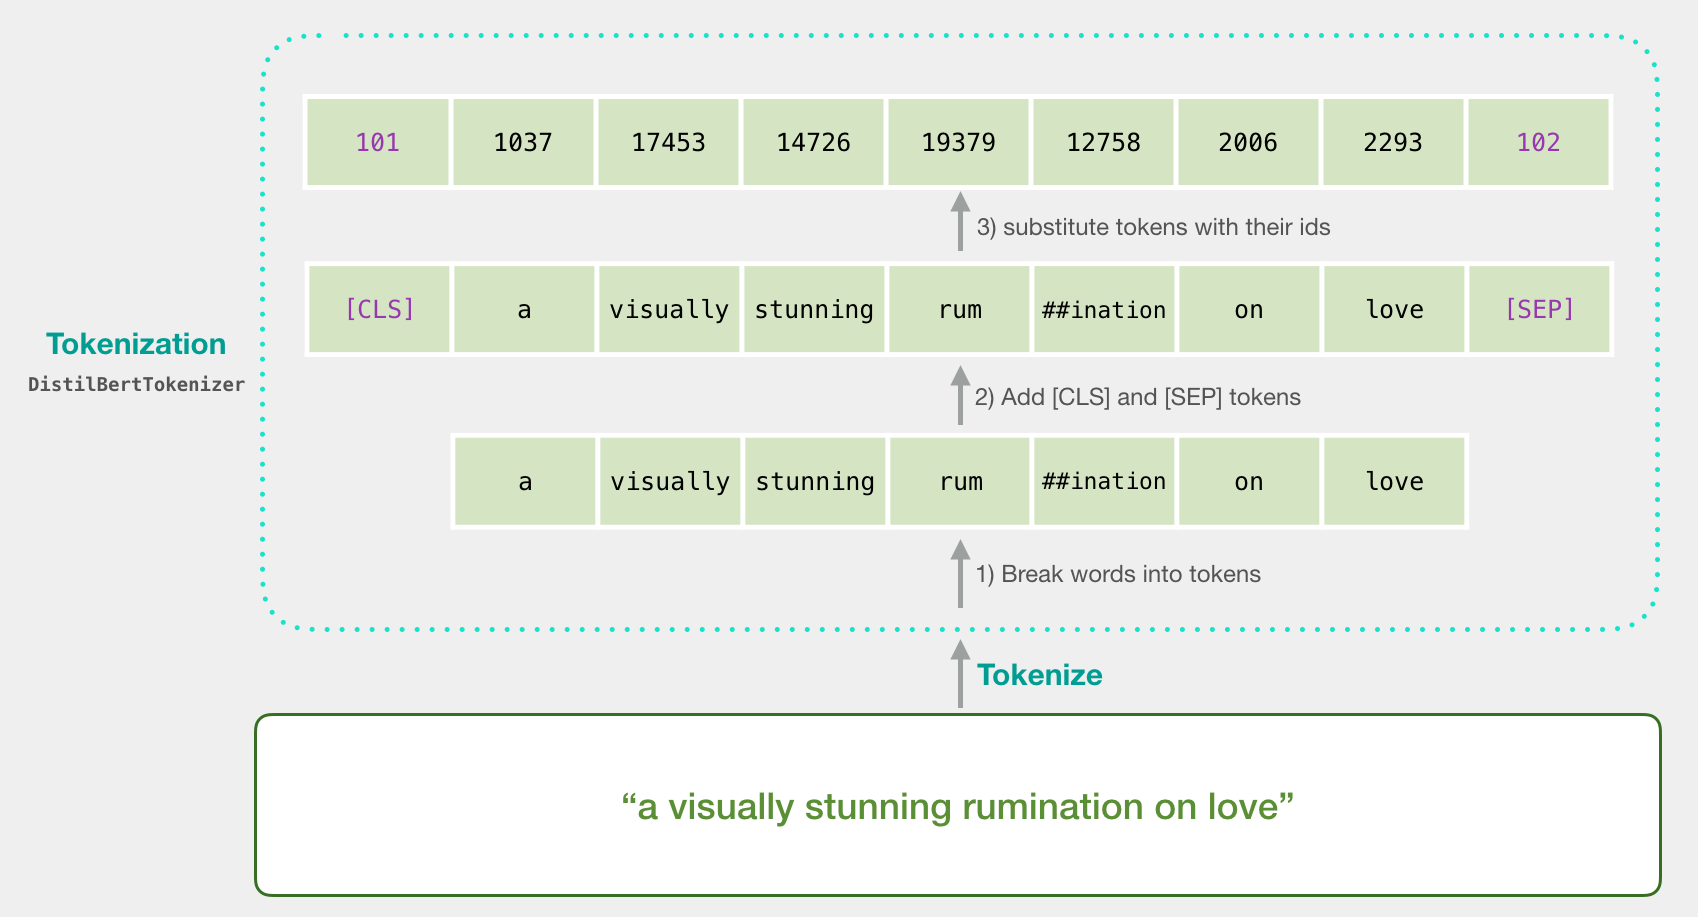
\includegraphics[width=0.8\textwidth]{fig/tokenization.png}
\caption{Full Scale Tokenization Example, where an English sentence is converted to tokens~\parencite{alammar_2019}.
}
\label{fig:tokenization}
\end{figure}

In order to limit the need for separate data files for both approaches, I chose not to add any other pre-processing to the text fields, such as removing duplicates or adding custom tokens. \acrshort{bert} relies on the spatial relationship between words in the sequence, and thus I wanted to maintain that order and only make structural changes when needed (see~\Cref{appendix:processing}). This was done in the actual training scripts themselves to reduce overhead. 

\section{Data Distribution}
\label{appendix:data-info}
The scraped data was converted into train, test, validation sets through a $70\%, 15\%, 15\%$ split. The fake-news corpus was then added only to the validation and test sets, making them much larger and more negative heavy.
% !TEX root = ../proceedings.tex
\begin{table}[h]
\centering
\begin{tabular}{|c|c|c|c|}
\hline
\multicolumn{4}{|c|}{Data Distribution} \\
\hline
Dataset & Total Length & $\#$ of Positive Examples & $\#$ of Negative Examples\\
\hline
Train & 100797 & 18598 & 82199 \\
Validation & 272447 & 4039 & 268348 \\
Test & 272448 & 4049 & 268399 \\
\hline
\end{tabular}
% BERT 466/1000
% rankfromsets 531/1000
% \vspace{1ex}
\caption{Dataset Breakdowns for training, test, and validation sets.}
\label{tab:data-breakdown}
\end{table}

\section{Training Scripts}
\label{appendix:training-scripts}
A collection of some of the most important training scripts that were utilized when performing the experiments.
\subsection{Evenly-Split Batch Generator}
For improved stability of the training process and because of the skewed nature of the datasets, I chose to feed in batches that had an even number of positive and negative labels. To do this, I created a subclass of the PyTorch Sampler \parencite{NEURIPS2019_9015}.
\begin{minted}{python}
import torch
import numpy as np
import torch.nn as nn

# Create batches with even splits
# positive samples in first half and negative examples in second half
class BatchSamplerWithNegativeSamples(torch.utils.data.Sampler):
    def __init__(self, pos_sampler, neg_sampler, batch_size, items):
        self._pos_sampler = pos_sampler
        self._neg_sampler = neg_sampler
        self._items = items
        assert (
            batch_size % 2 == 0
        ), "Batch size must be divisible by two for negative samples."
        self._batch_size = batch_size

    def __iter__(self):
        batch, neg_batch = [], []
        neg_sampler = iter(self._neg_sampler)
        for pos_idx in self._pos_sampler:
            batch.append(pos_idx)
            neg_idx = pos_idx
            # keep sampling until we get a true negative sample
            while self._items[neg_idx] == self._items[pos_idx]:
                try:
                    neg_idx = next(neg_sampler)
                except StopIteration:
                    neg_sampler = iter(self._neg_sampler)
                    neg_idx = next(neg_sampler)
            neg_batch.append(neg_idx)
            if len(batch) == self._batch_size // 2:
                batch.extend(neg_batch)
                yield batch
                batch, neg_batch = [], []
        return

    def __len__(self):
        return len(self._pos_sampler) // self._batch_size

\end{minted}

\subsection{RankFromSets Batched Predictions}
\begin{minted}{python}
@torch.no_grad()
def calculate_batched_predictions(batch, model, device, target):
    model.eval()
    (publications, articles, word_attributes, 
    attribute_offsets, real_labels) = batch
    publication_set = [target] * len(real_labels)
    publication_set = torch.tensor(publication_set, dtype=torch.long)
    publication_set = publication_set.to(device)
    articles = articles.to(device)
    word_attributes = word_attributes.to(device)
    attribute_offsets = attribute_offsets.to(device)
    logits = model(publication_set, articles, 
    			   word_attributes, attribute_offsets)
    final_logits = logits.cpu().numpy()
    return final_logits
\end{minted}

\subsection{BERT Batched Predictions}
\begin{minted}{python}
@torch.no_grad()
def calculate_batched_predictions(batch, model, device, target):
    model.eval()
    (word_attributes, attention_masks, 
    word_subset_counts, real_labels) = batch
    word_attributes = word_attributes.to(device)
    attention_masks = attention_masks.to(device)
    logits = model(word_attributes, attention_mask=attention_masks)[0]
    final_logits = np.squeeze(logits.cpu().numpy())
    return final_logits
\end{minted}

\subsection{Recall Calculation}
\begin{minted}{python}
@torch.no_grad()
def calculate_recall(
    dataset, indices, recall_value=1000, 
    target_publication, version, writer, step,
):
    rev_indices = indices[::-1]
    correct_10 = 0
    correct_big = 0
    for i in range(recall_value):
        if dataset[rev_indices[i]]["model_publication"] == target_publication:
            if i < 10:
                correct_10 += 1
            correct_big += 1
    print(f"{version} Performance: Step - {step}")
    print(f"Top 10: {correct_10*10} %")
    print(
        f"Top {str(recall_value)}: {(correct_big*100)/recall_value} %"
    )
    print("--------------------")
    writer.add_scalar(f"{version}/Top-10", correct_10, step)
    writer.add_scalar(f"{version}/Top-{recall_value}", correct_big, step)
    return correct_big
\end{minted}

\section{Permission Email}
\label{appendix:permission}
\subsection{Email Sent to Mr. Uri Bram of The Browser}

Hello Mr. Bram,

I am currently working on a machine-learning computer science paper for school. My goal is to compare models in their ability to predict "quality" writing. There is a general scarcity in terms of positive data in this space, and I was wondering if I could utilize your Browser archives. The data will not be published or utilized in any external manner. 

Thanks in advance, \\
\blackout{Rohan}

\subsection{Permission Received from Mr. Uri Bram of The Browser}

Dear \blackout{Rohan},

Thank you so much for your kind email. It sounds like a great project and we would be happy for you to use the Browser archive. Please let me know if I can be of any further assistance.

Best,

Uri Bram
CEO, The Browser Ltd